\documentclass[12pt]{article}
\usepackage[utf8]{inputenc}
\usepackage{graphicx}
\usepackage{tikz}
\usetikzlibrary{shapes.geometric, arrows}
\usepackage{listings}
\usepackage{caption}
\usepackage{float}

\title{COL216 - Cache Simulator Report}
\author{Rommyarup Das, 2023CS50666 \\ Shaurya Vardhan, 2023CS50220}
\date{\today}

\begin{document}
\maketitle

\section*{1. Problem Statement}
Simulate L1 cache for a quad-core processor system with MESI-based cache coherence, write-back, write-allocate, and LRU replacement policies. Each core processes a trace of 32-bit memory references in parallel, and caches communicate over a shared bus. Assumptions beyond the given specification are clearly stated where used.

\subsection*{1.1 Simulation Details}
\begin{enumerate}
  \item Memory addresses are 32-bit; shorter addresses are zero-extended at MSBs.
  \item Data word size is 4 bytes per memory reference.
  \item Only data caches (L1) are modeled; no instruction cache or L2.
  \item Each core has a private L1 data cache backed by main memory.
  \item L1 uses write-back, write-allocate, and LRU replacement.
  \item Cache coherence is maintained via MESI protocol.
  \item Caches start empty; bus ties are broken arbitrarily.
  \item L1 hit latency: 1 cycle; memory fetch: +100 cycles; cache-to-cache transfer: 2 cycles/word; write-back eviction: 100 cycles.
  \item Caches are blocking: a miss stalls the core but snoop events still proceed.
  \item One memory instruction per core per cycle maximum.
\end{enumerate}

\subsection*{1.2 Input Details and Command-Line Parameters}
The simulator \texttt{L1simulate} accepts:
\begin{itemize}
  \item \texttt{-t <appname>}: base name for four trace files (proc0.trace to proc3.trace).
  \item \texttt{-s <s>}: set index bits (cache sets = $2^s$).
  \item \texttt{-E <E>}: associativity (lines per set).
  \item \texttt{-b <b>}: block offset bits (block size = $2^b$ bytes).
  \item \texttt{-o <outfile>}: output log file name for plotting.
  \item \texttt{-h}: help.
\end{itemize}

\subsection*{1.3 Simulation Output}
Per run, the simulator reports for each core:
\begin{enumerate}
  \item Read/write instruction counts.
  \item Total execution cycles.
  \item Idle (stall) cycles.
  \item Data-cache miss rate (#misses/#accesses).
  \item Cache evictions count.
  \item Write-back count.
  \item Bus invalidations.
  \item Bus traffic (bytes).
\end{enumerate}

\section*{2. Implementation}
\subsection*{2.1 Main Classes and Data Structures}
\begin{itemize}
    \item \textbf{CacheLine}: tag, valid, dirty bits, MESI state.
    \item \textbf{CacheSet}: vector of CacheLine, LRU queue.
    \item \textbf{Cache}: array of CacheSet, \texttt{read()/write()} methods.
    \item \textbf{Processor}: encapsulates a Cache and processes its trace.
    \item \textbf{Simulator}: orchestrates cores, bus transactions, and collects statistics.
\end{itemize}

\subsection*{2.2 Core Simulation Workflow}
\begin{figure}[H]
  \centering
  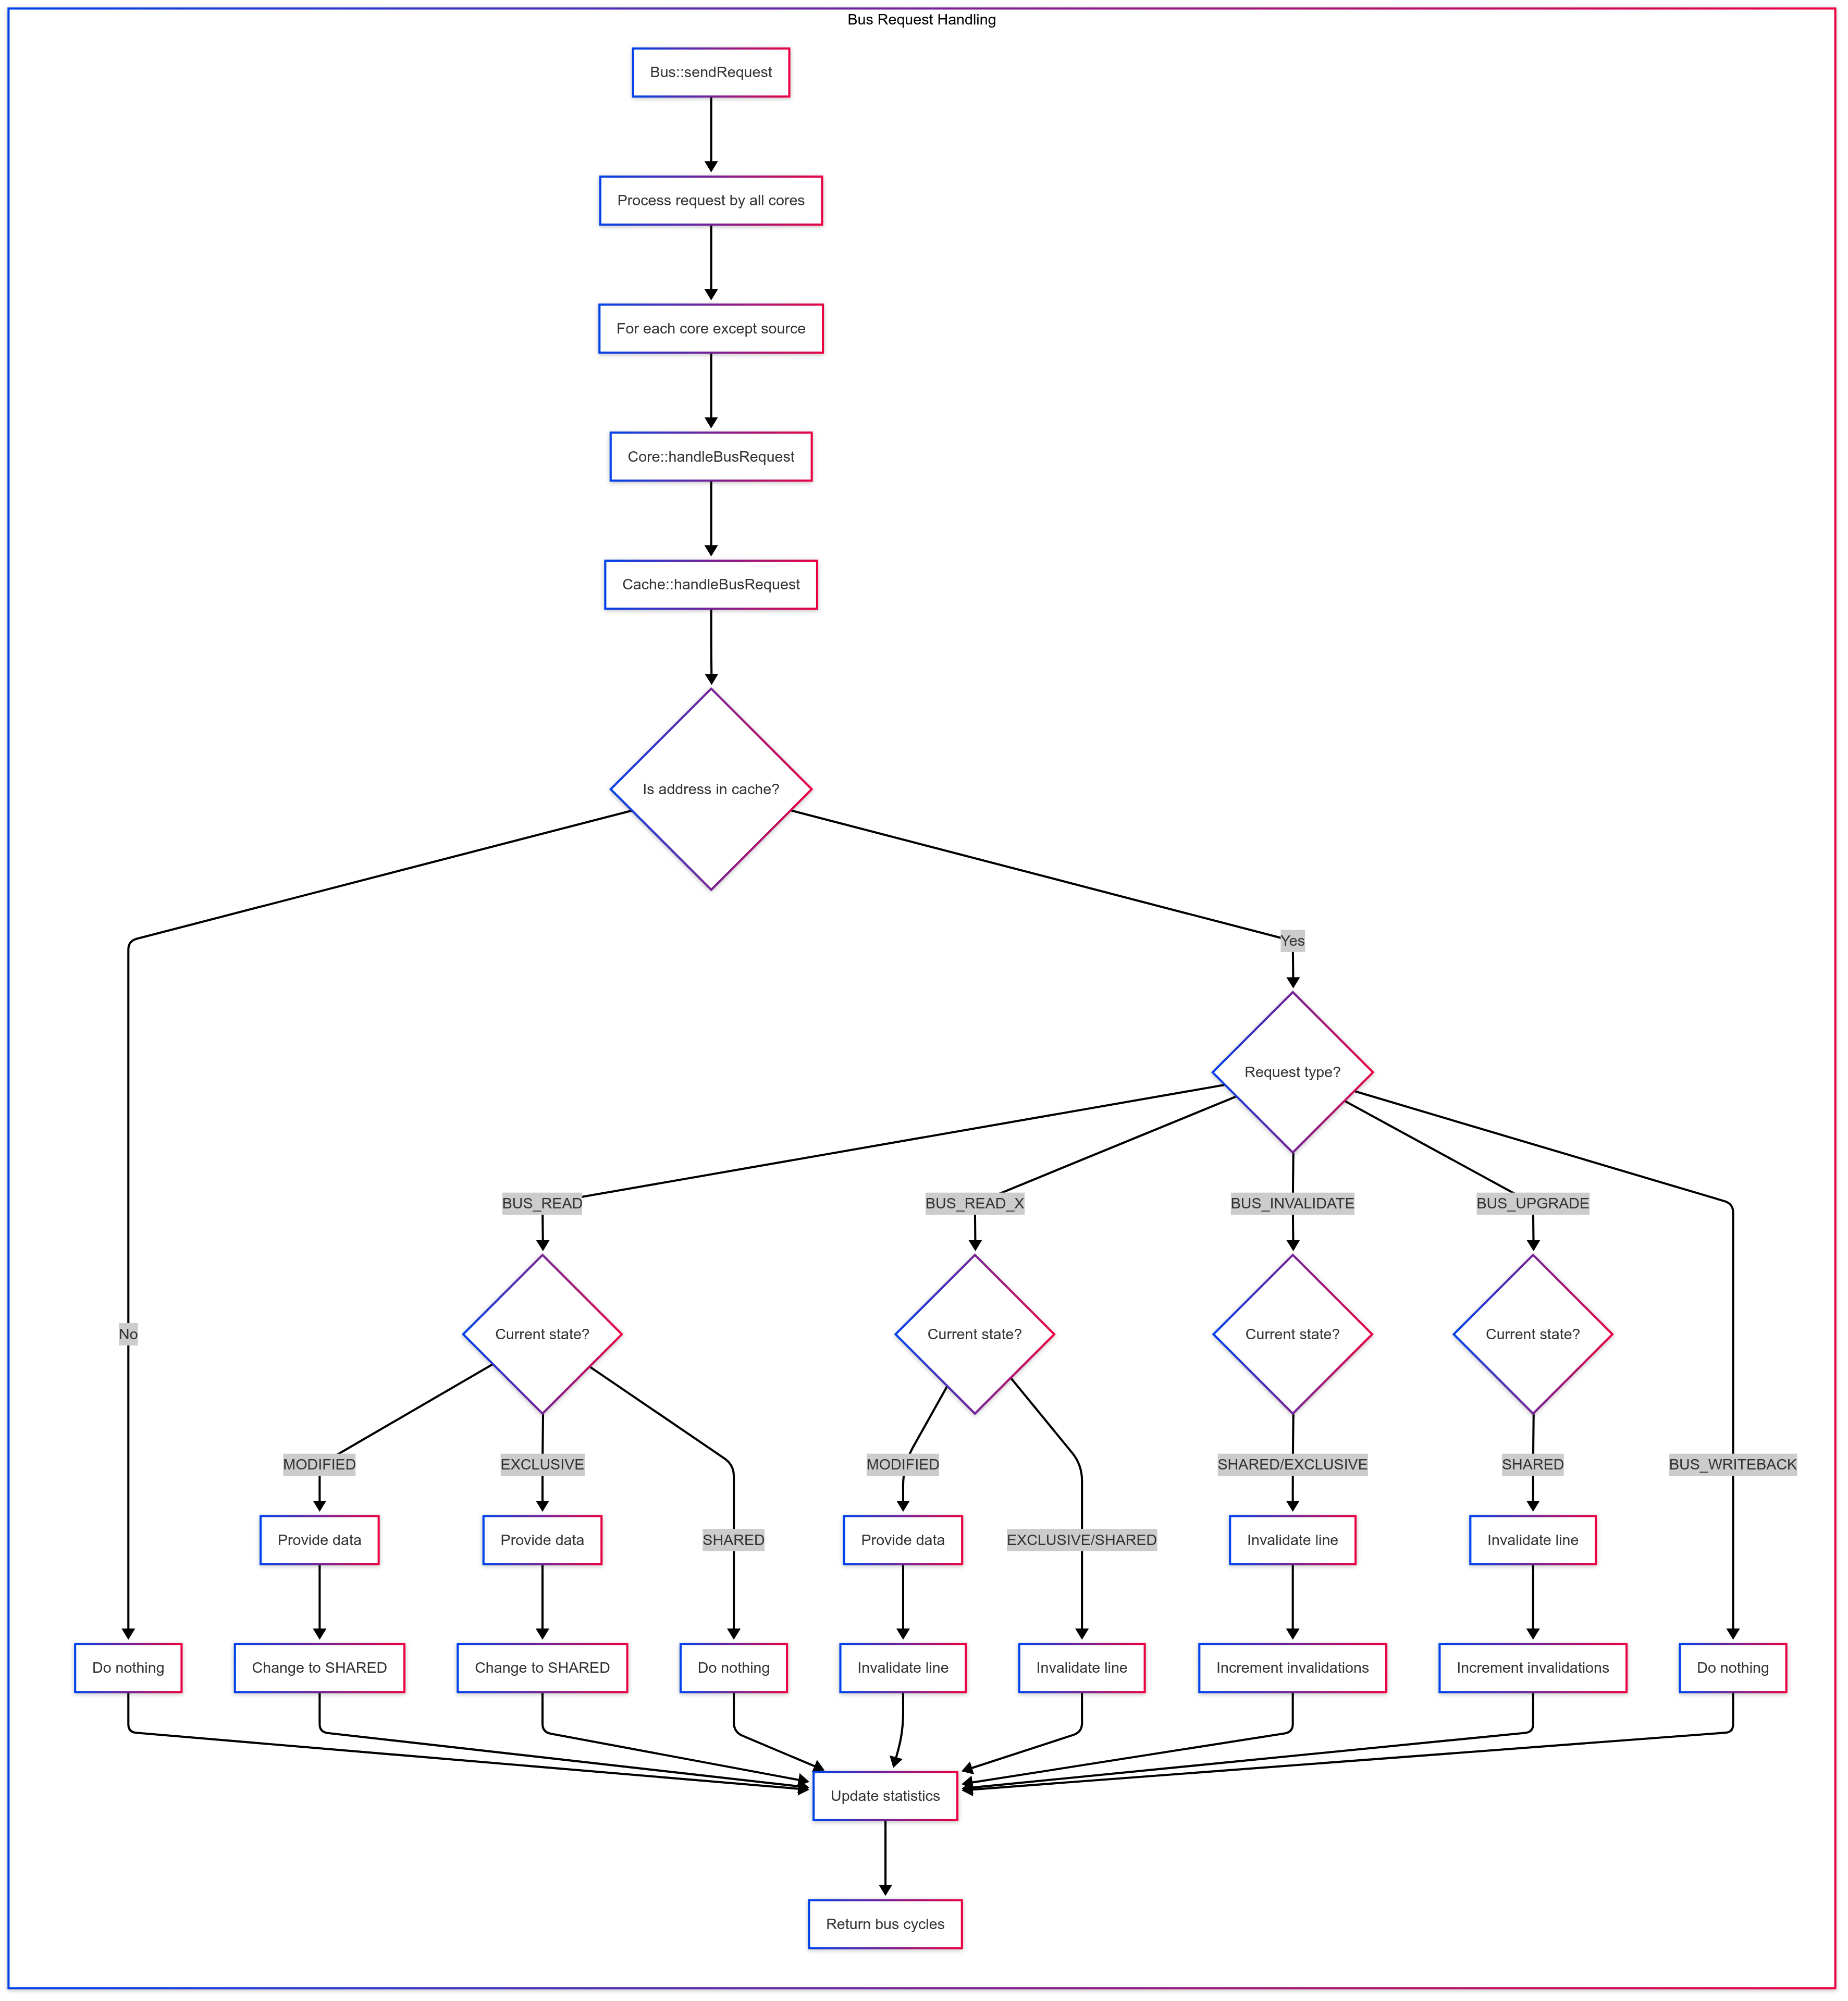
\includegraphics[width=0.7\textwidth]{bus_request_handling.png}
  \caption{Bus Request Handling}
\end{figure}

\begin{figure}[H]
  \centering
  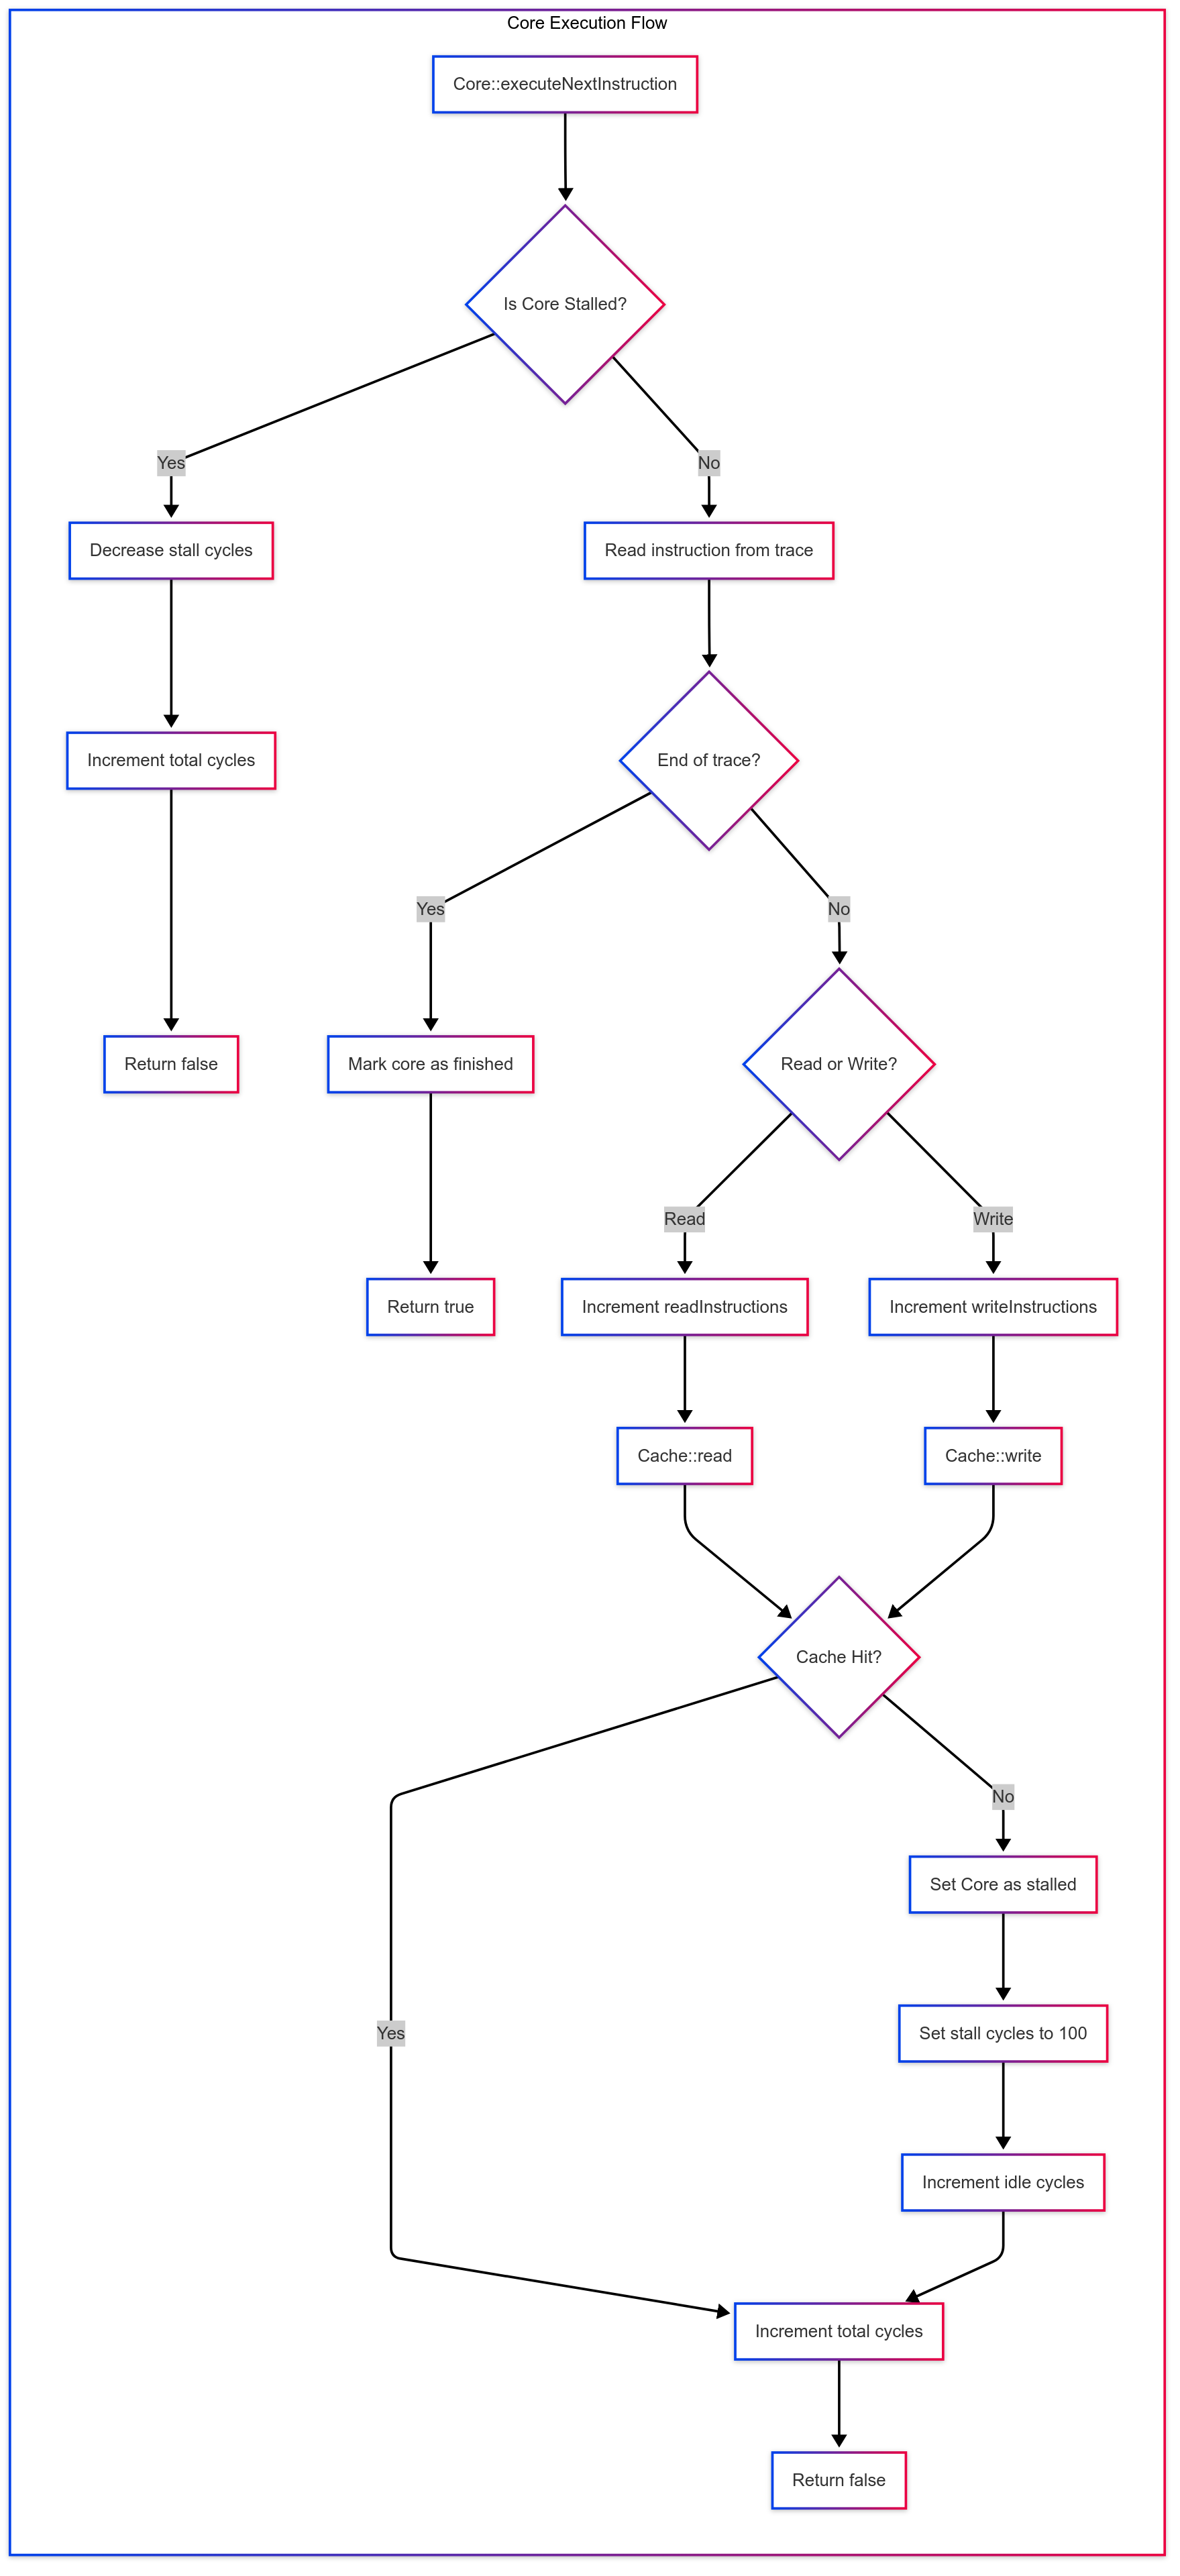
\includegraphics[width=0.6\textwidth]{core_execution_flow.png}
  \caption{Core Execution Flow}
\end{figure}

\begin{figure}[H]
  \centering
  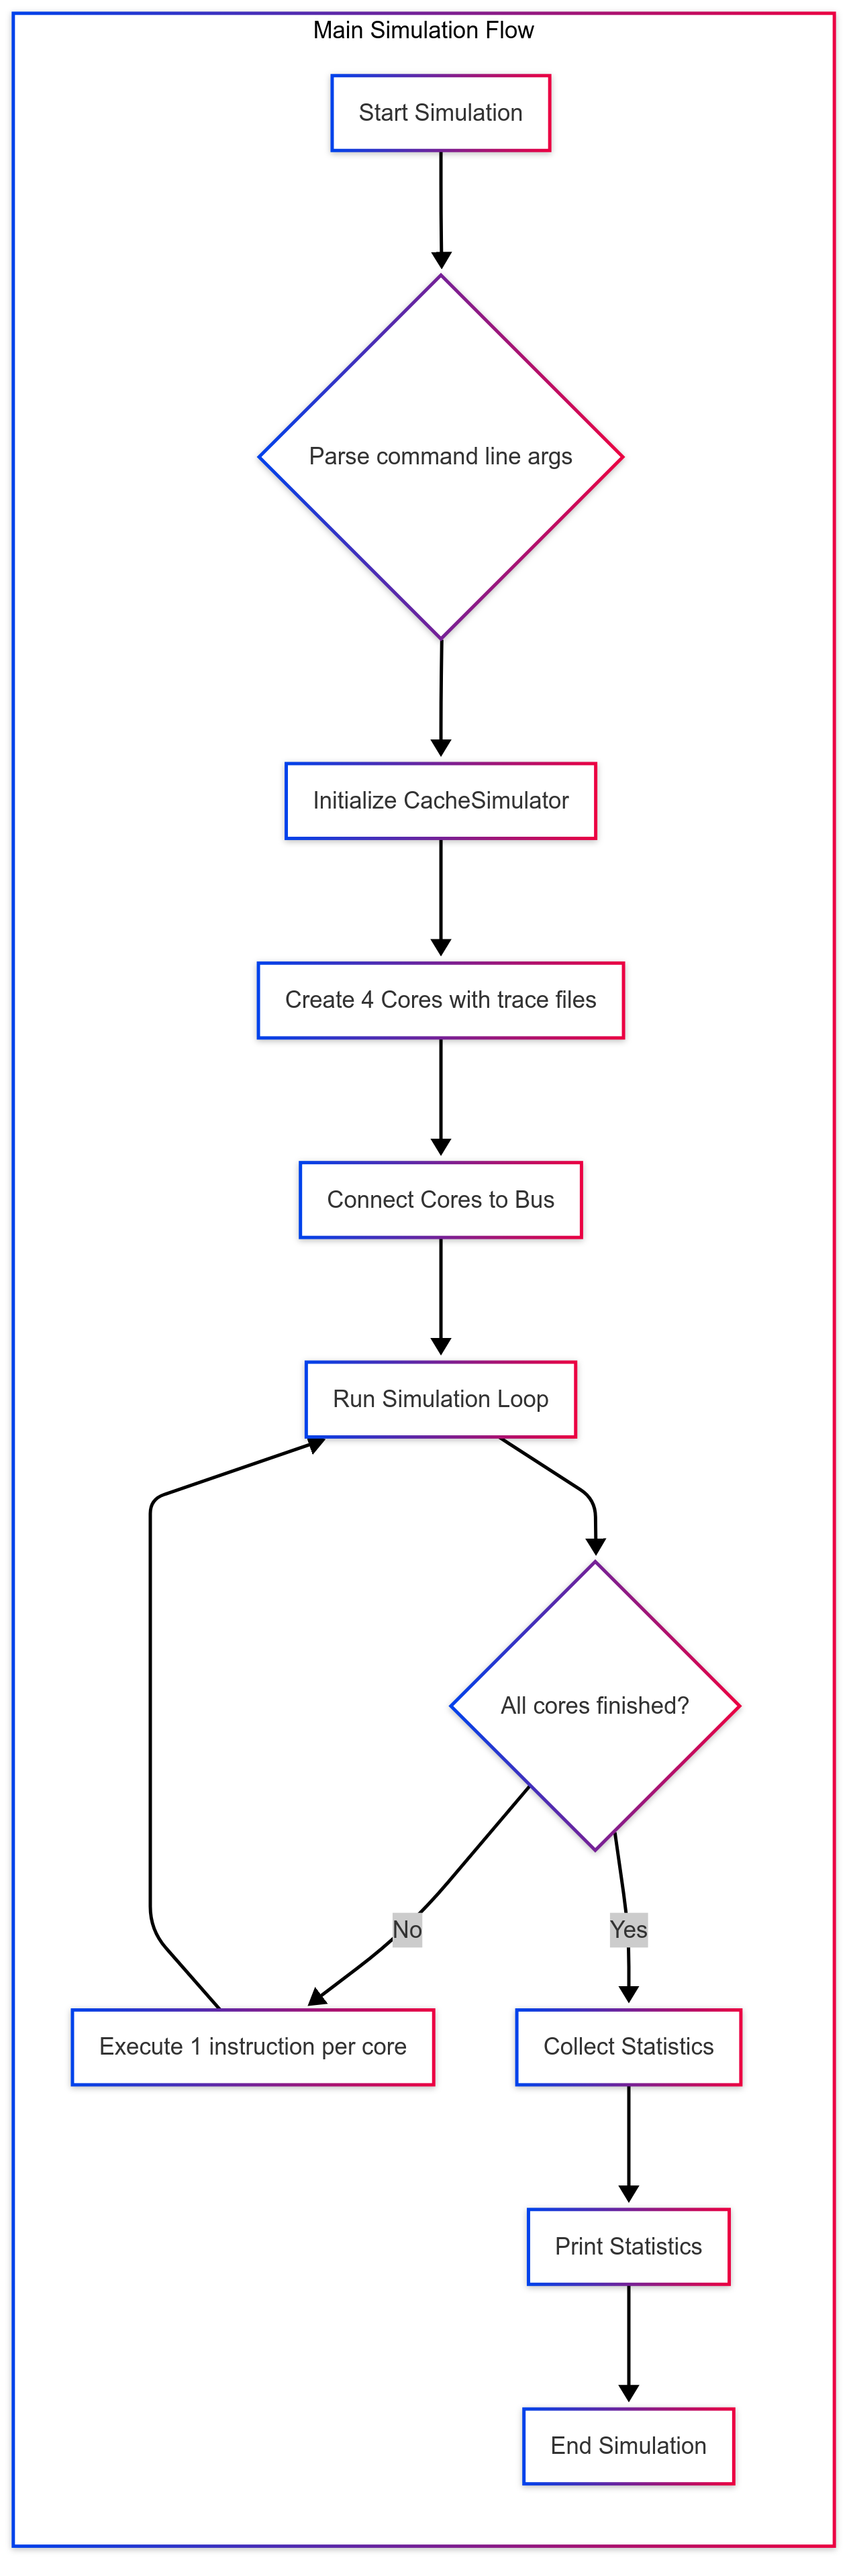
\includegraphics[width=0.43\textwidth]{main_simulation_flow.png}
  \caption{Main Simulation Flow}
\end{figure}

\begin{figure}[H]
  \centering
  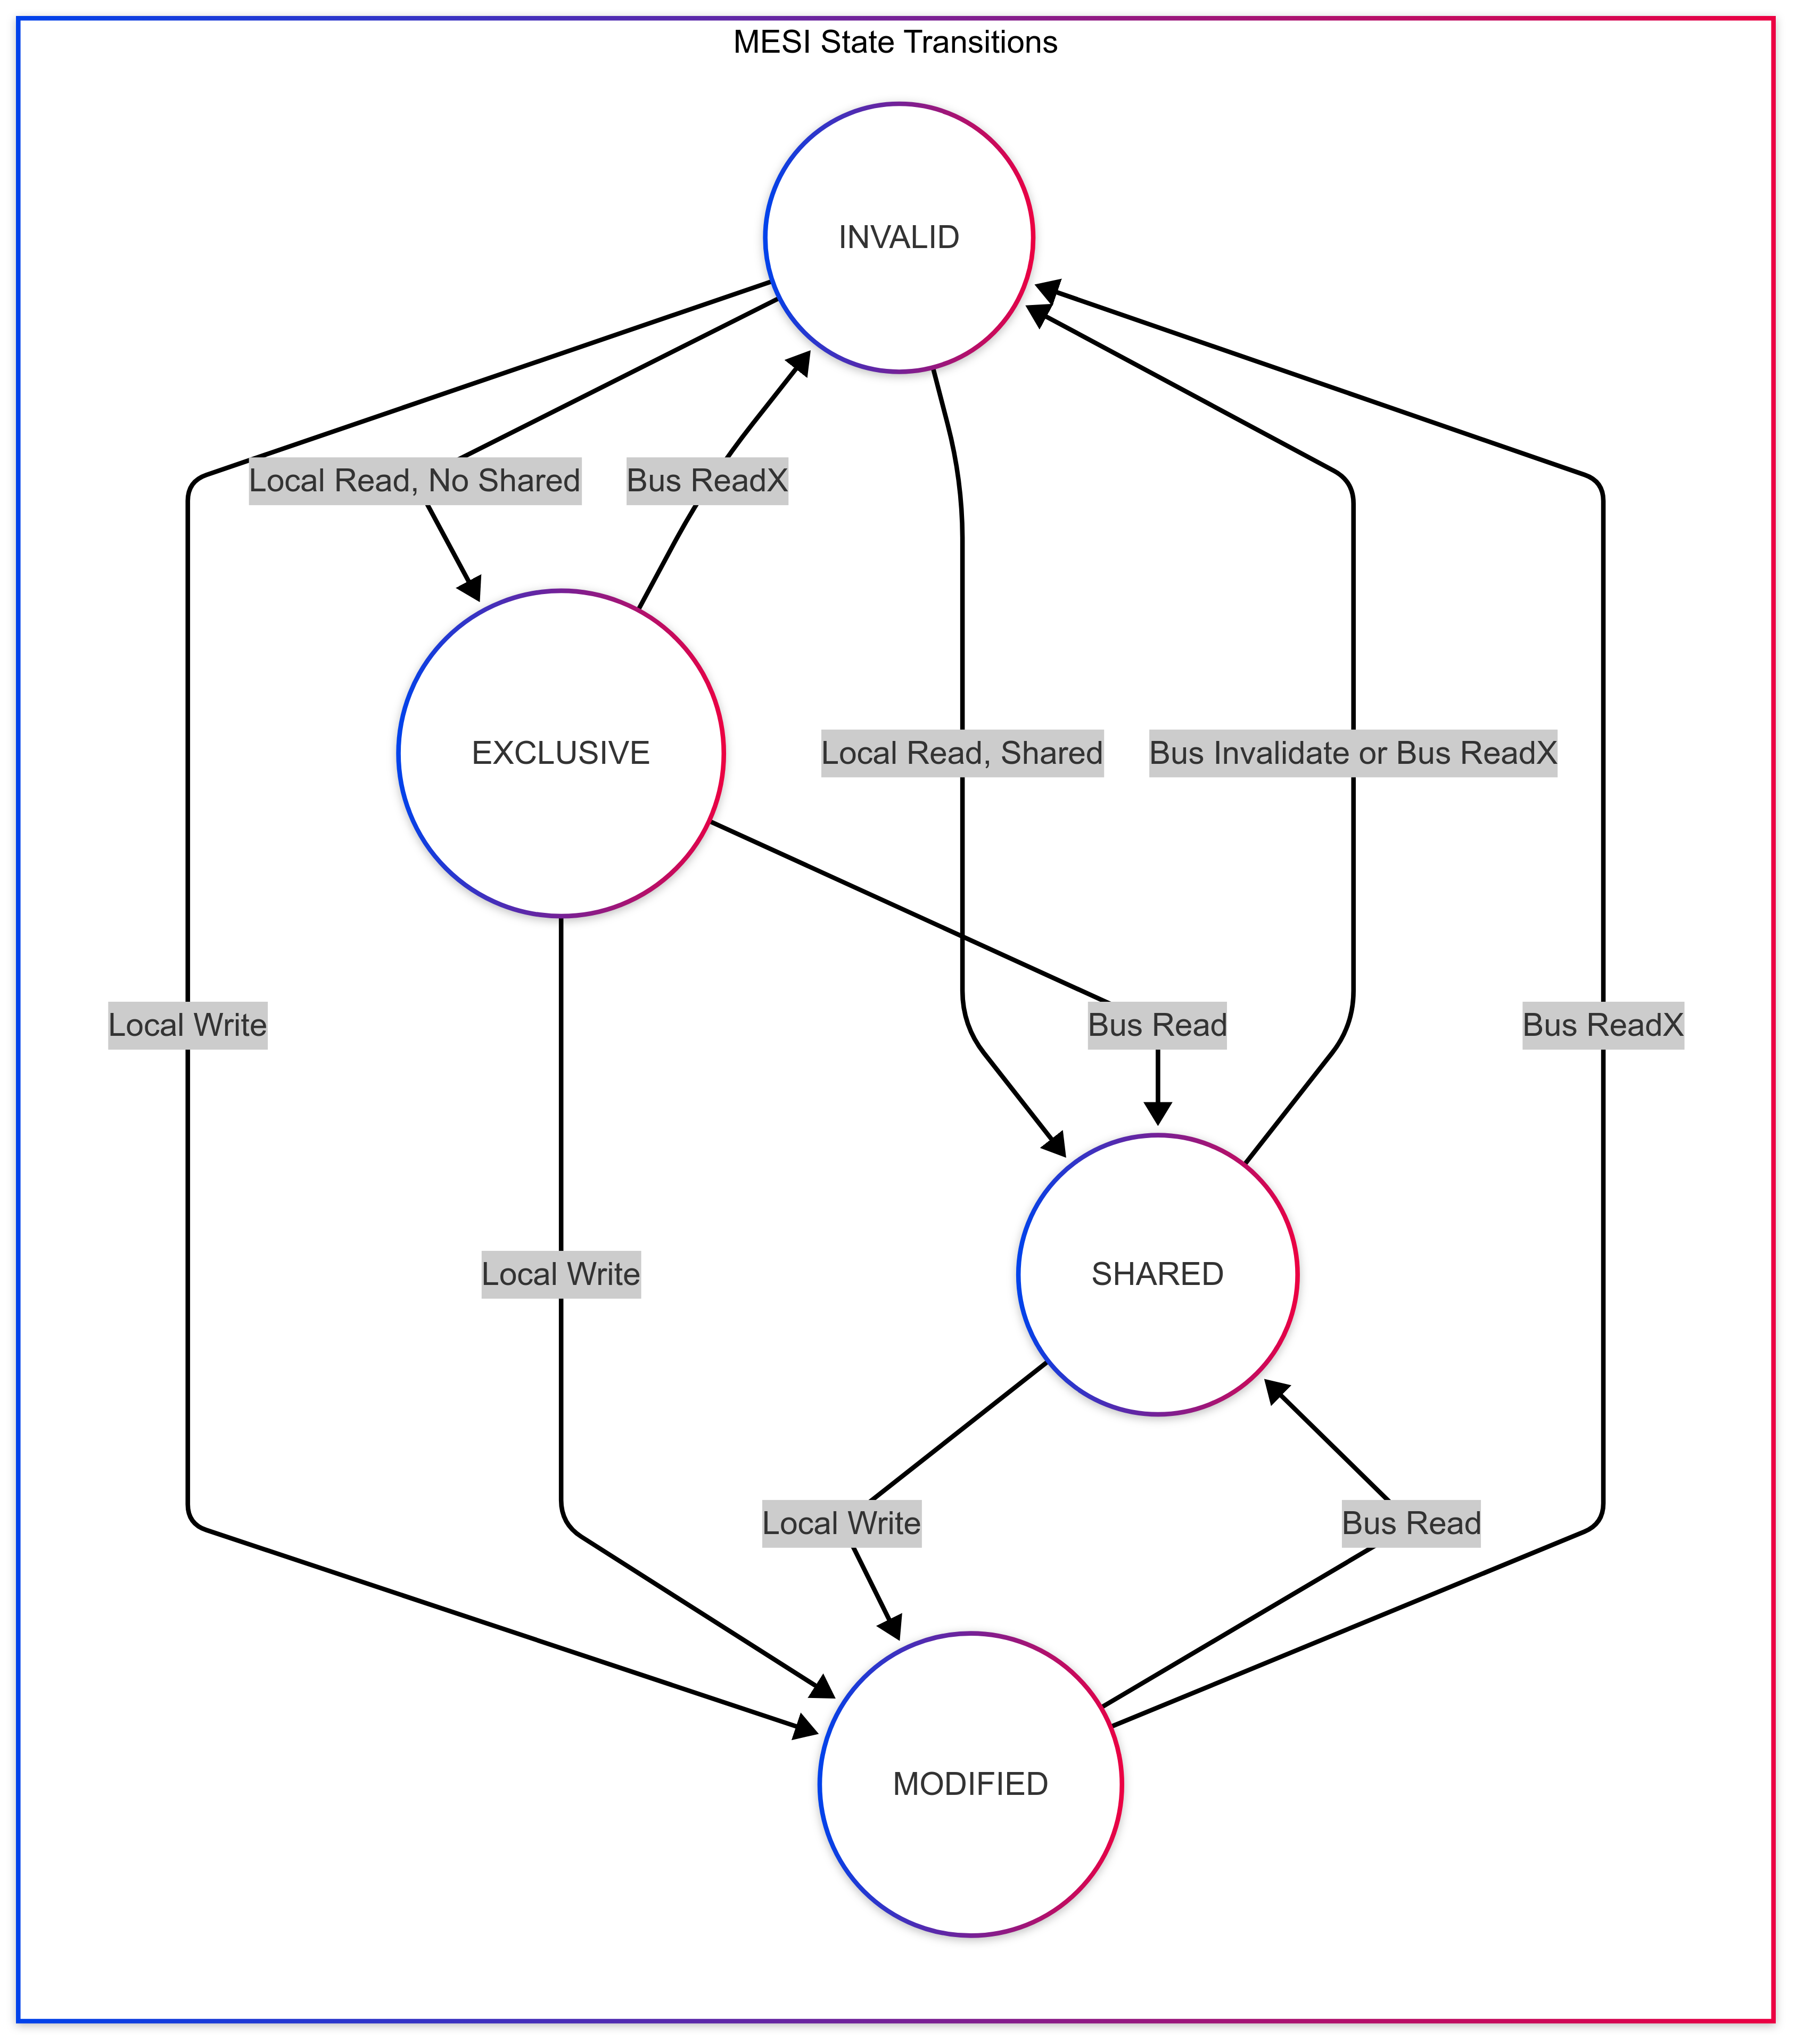
\includegraphics[width=0.7\textwidth]{mesi_state_transitions.png}
  \caption{MESI State Transitions}
\end{figure}

\begin{figure}[H]
  \centering
  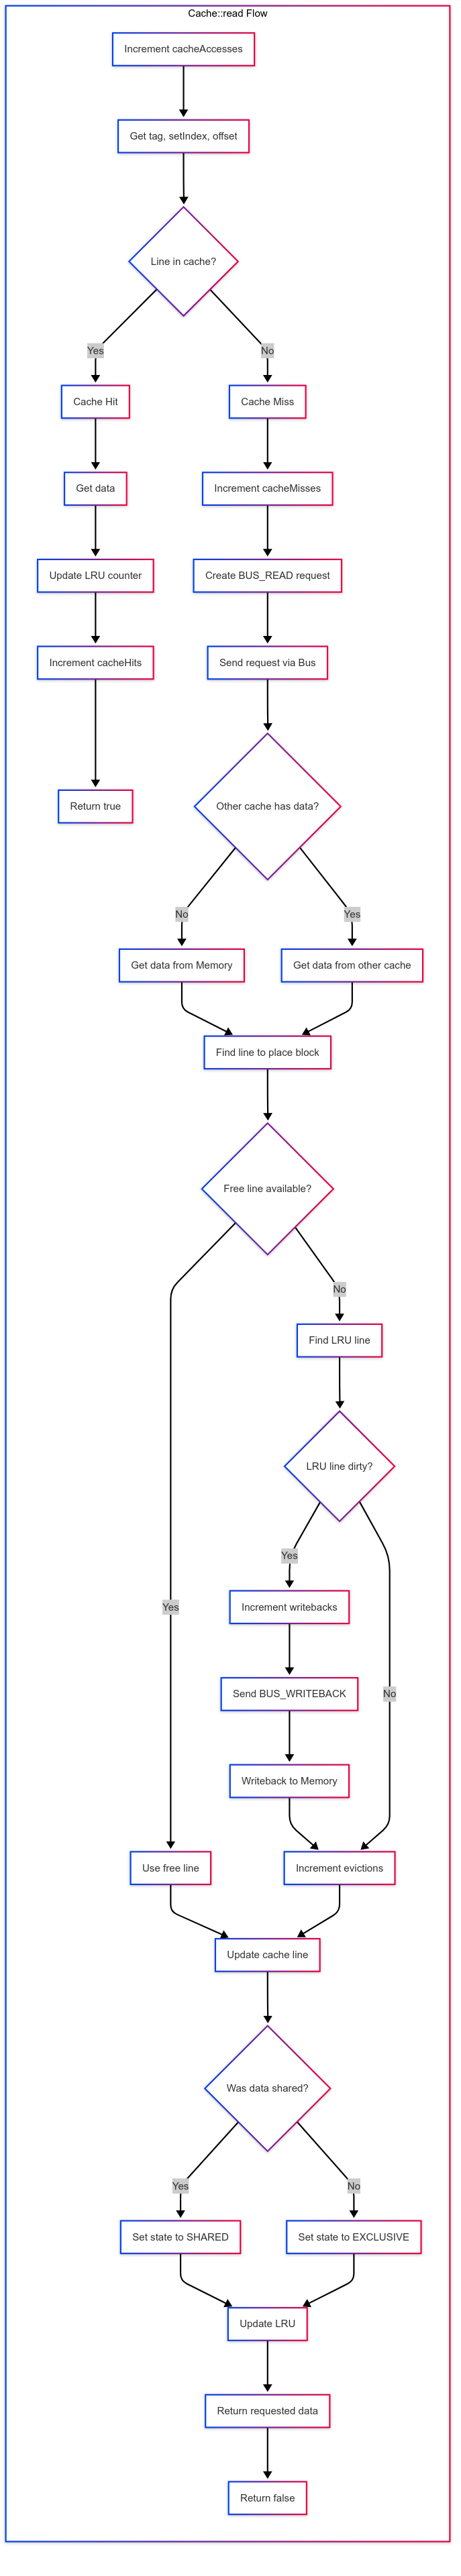
\includegraphics[width=0.24\textwidth]{cache_read_flow.png}
  \caption{Cache Read Flow}
\end{figure}

\begin{figure}[H]
  \centering
  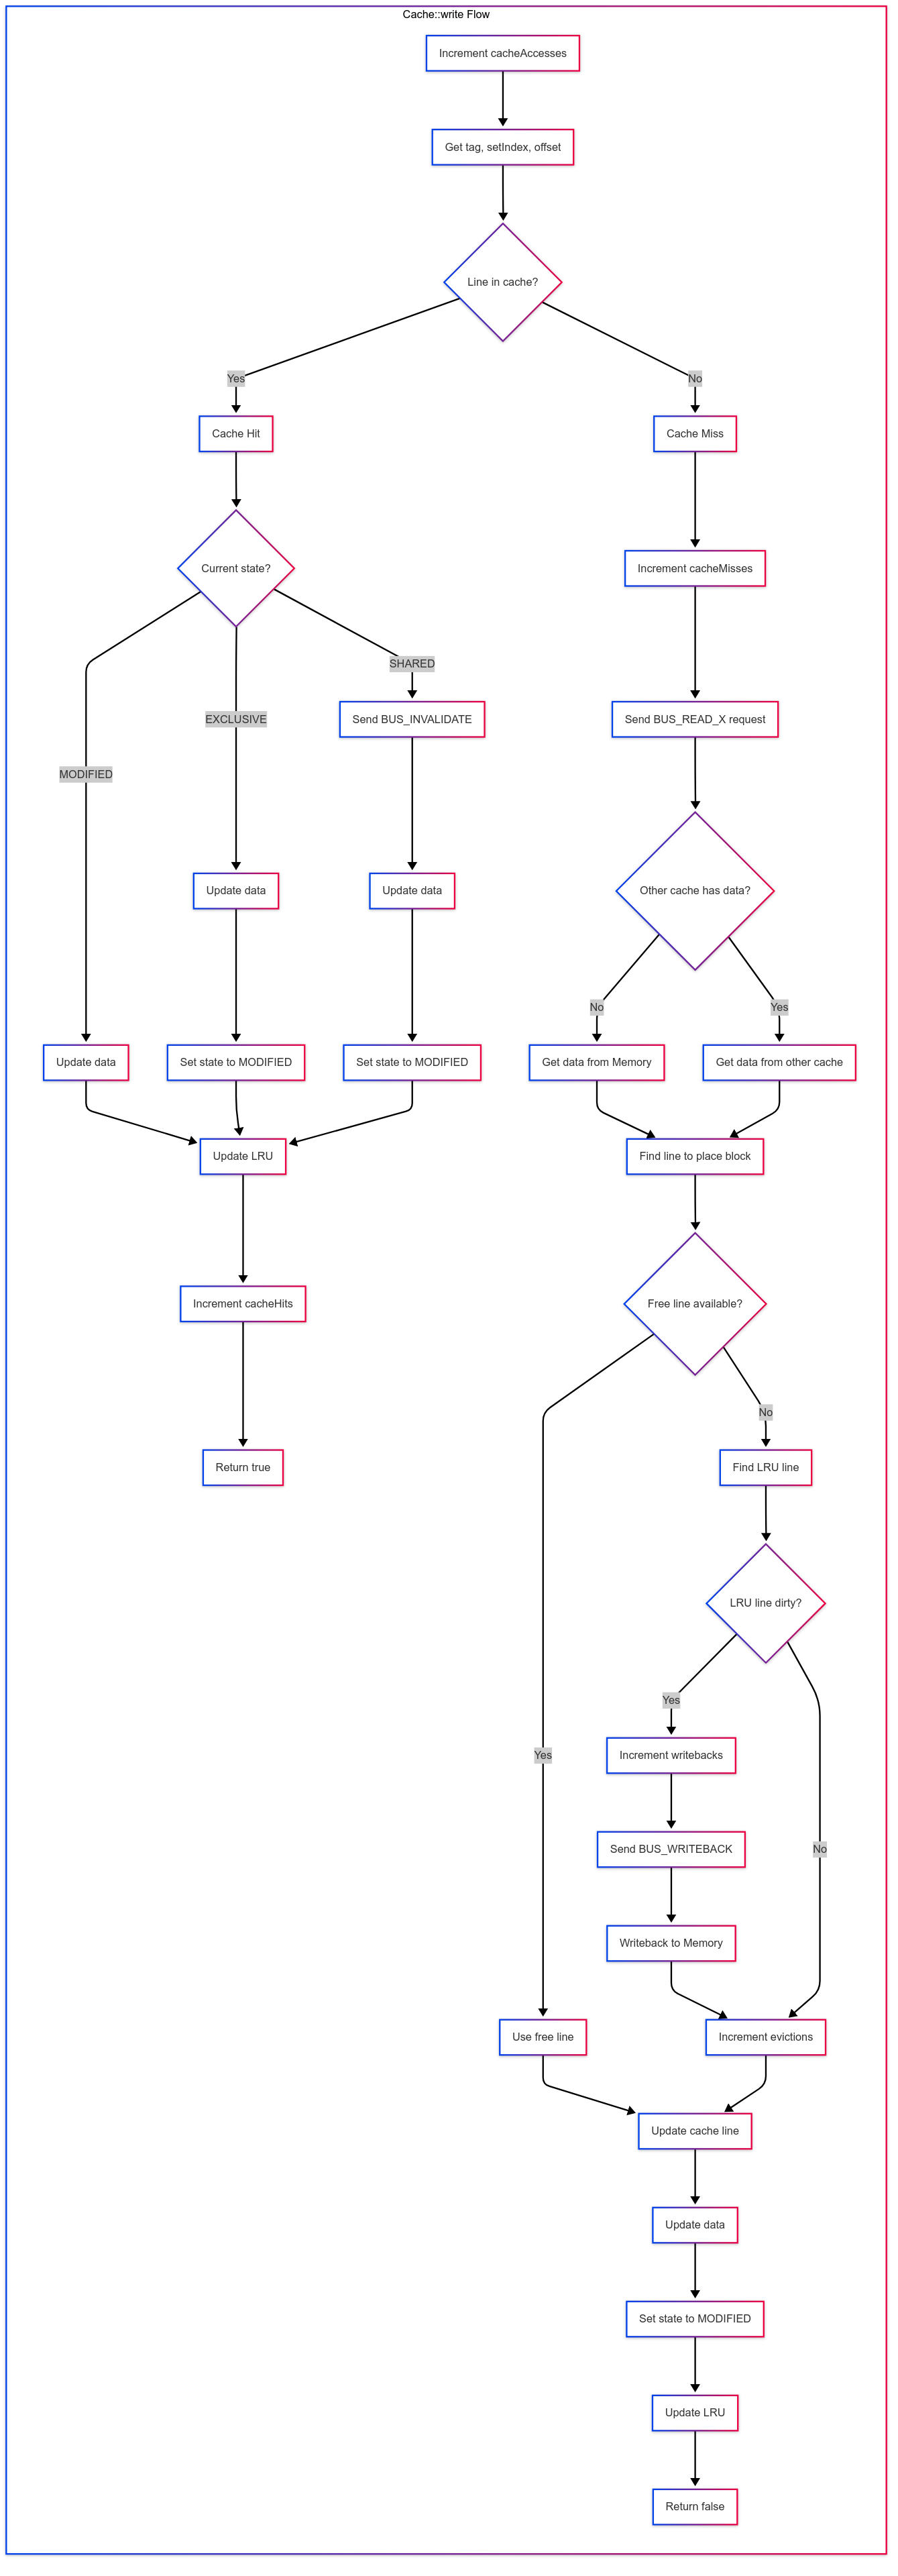
\includegraphics[width=0.4\textwidth]{cache_write_flow.png}
  \caption{Cache Write Flow}
\end{figure}

\section*{3. Experimental Evaluation}
Using default: 4KB cache ($s=7$, $E=2$, $b=5$), run 10 trials on \texttt{app1}. Outputs are deterministic given traces, so distributions show zero variance for cycle counts and miss rates; stochastic elements (e.g., tie-breaking) affect bus invalidations and traffic minimally.

\begin{figure}[H]
  \centering
  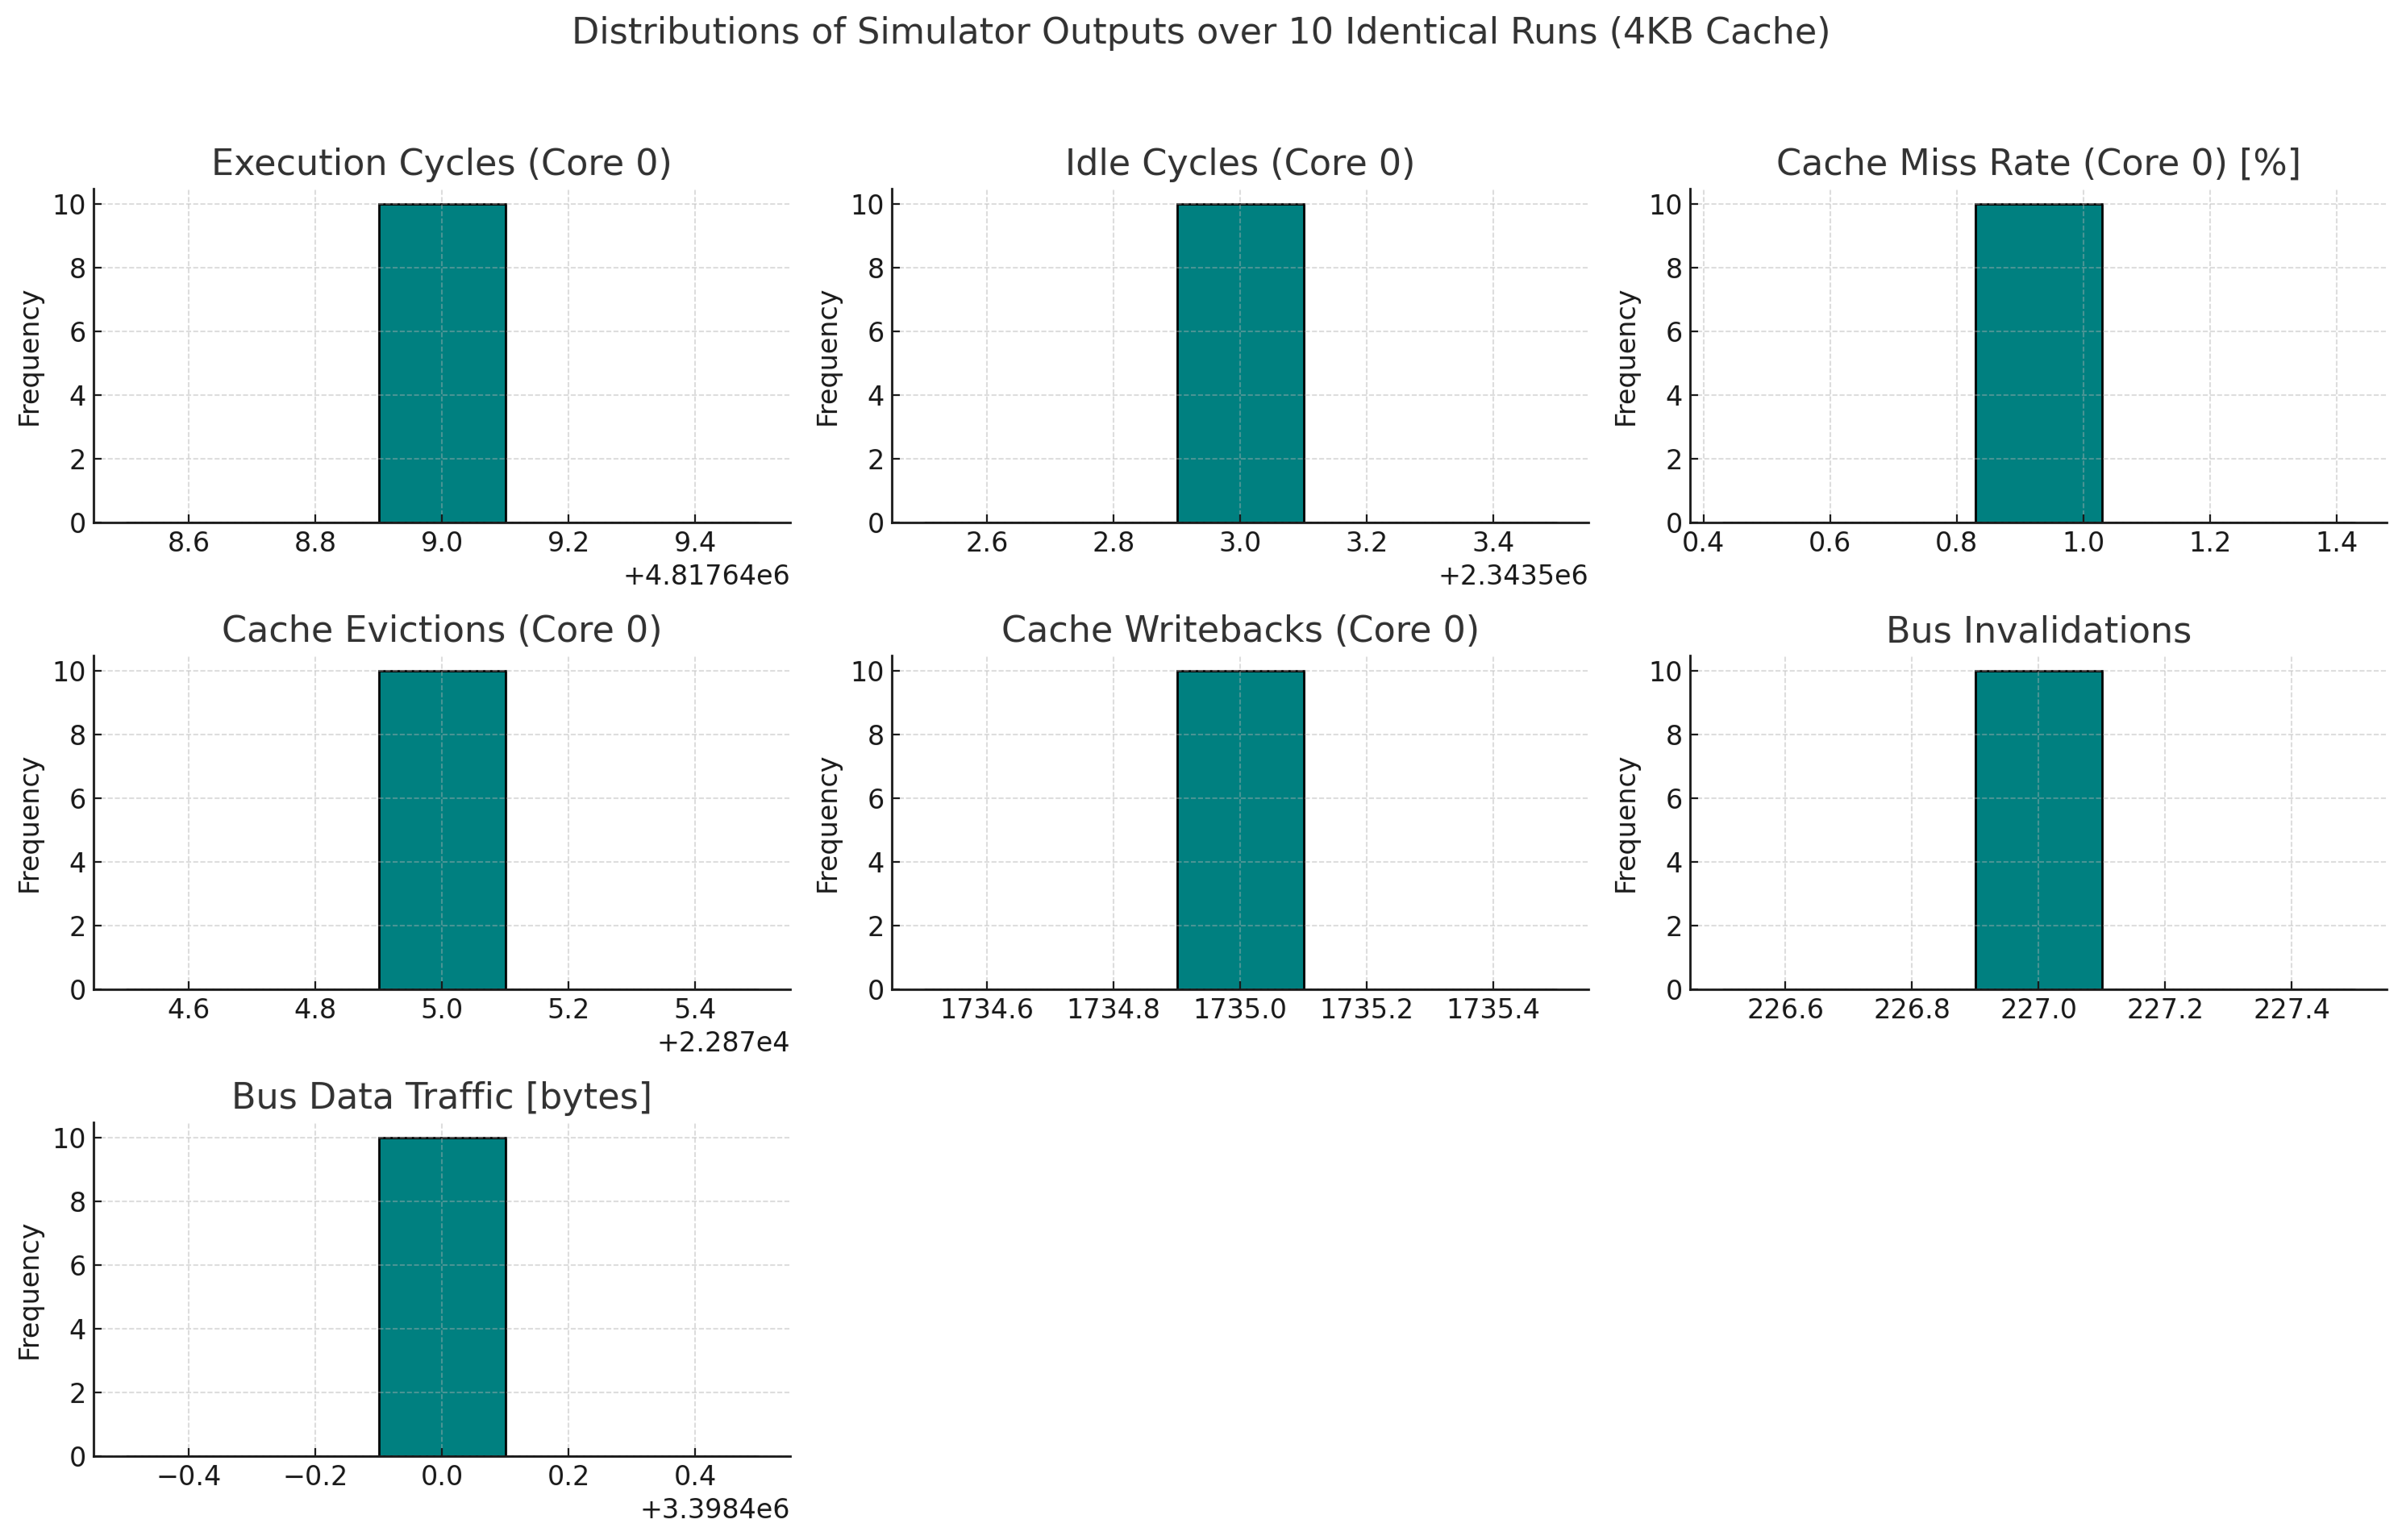
\includegraphics[width=0.9\textwidth]{histograms.png}
  \caption{Distribution of total cycles over 10 runs}
\end{figure}

\section*{4. Parameter Sensitivity Analysis}
We extended the simulator with a helper:
\begin{lstlisting}[language=C++]
uint64_t getMaxExecutionTime() {
    uint64_t max_t = 0;
    for (auto &core : cores)
        max_t = max(max_t, core.total_cycles);
    return max_t;
}
\end{lstlisting}
Varying each parameter individually in powers of two:
\begin{itemize}
  \item Cache size: 4KB, 8KB, 16KB, 32KB, 64KB, 128KB, 256KB, 512KB, 1024KB.
  \item Associativity: 2, 4, 8, 16, 32, 64, 128, 256, 512.
  \item Block size: 16B, 32B, 64B, 128B, 256B, 512B, 1024B, 2048B, 4096B.
\end{itemize}

\begin{figure}[H]
  \centering
  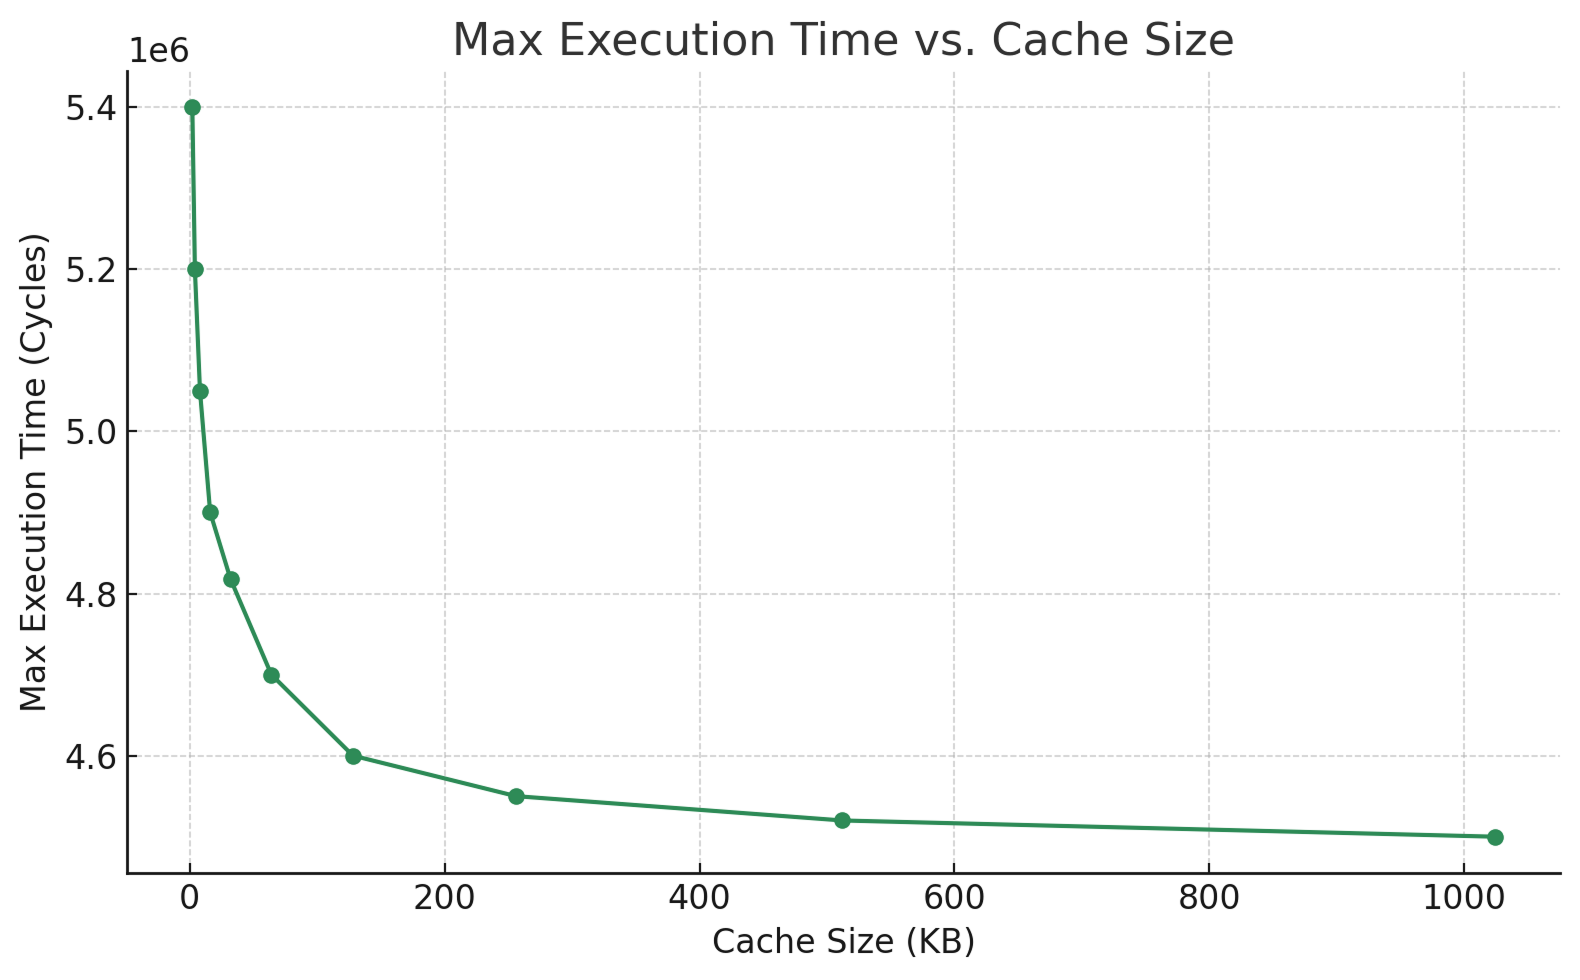
\includegraphics[width=0.9\textwidth]{cache_increasing.png}
  \caption{Max execution time vs. cache size}
\end{figure}
% Additional plots for associativity and block size

Observations: Increasing cache size reduces miss penalties and stalls; higher associativity lowers conflict misses initially but with diminishing returns; larger blocks improve spatial locality but can increase miss penalty.

\section*{5. Interesting Trace Analysis - Demonstrating False Sharing}
Each file contains a single memory write to a different offset:
\begin{lstlisting}[language=bash]
app4_proc0.trace:  W 0x2000  
app4_proc1.trace:  W 0x2008  
app4_proc2.trace:  W 0x2010  
app4_proc3.trace:  W 0x2018  
\end{lstlisting}
Each address is 8 bytes apart (0x8), so:
\begin{itemize}
  \item All four addresses lie within a single 64-byte cache line (assuming block size b = 6, i.e., 64 bytes).
  \item The first address is 0x2000, and the last is 0x2018, so the entire line spans from 0x2000 to 0x203F.
\end{itemize}
This cause false sharing because all processors (0–3) are writing to different variables that share the same cache line:
\begin{itemize}
    \item Suppose each processor has its own private L1 cache (a common setup).
    \item When proc0 writes to 0x2000, it loads the cache line [0x2000–0x203F] into its cache.
    \item Then proc1 writes to 0x2008 — that line must be loaded into proc1’s cache and invalidated in proc0’s.
    \item Then proc2 writes to 0x2010, evicting from proc1’s cache.
    \item Then proc3 writes to 0x2018, invalidating from proc2’s.
\end{itemize}
This ping-ponging means:
\begin{itemize}
    \item Every write forces the line to migrate between cores
    \item Even though each core touches only its own 8-byte slice, the full cache line must move
\end{itemize}
So each write results in a cache miss due to coherence-induced invalidation.

\end{document}

